% =============================================
% =============================================
% Document class: Article
\documentclass[ a4paper, twoside, 11pt]{article}
% Packages: LaTeX (Depth-1)
\usepackage[ vlined, linesnumbered, ruled]{algorithm2e}
\usepackage{ amsfonts, amsmath, amssymb, amsthm}
\usepackage[ titletoc, title]{appendix}
\usepackage{ bbm}
\usepackage{ color}
\usepackage{ dsfont}
\usepackage{ enumitem}
\usepackage{ graphicx}
\usepackage{ fancyhdr, float, fullpage}
\usepackage{ hyperref}
\usepackage{ lastpage, latexsym, lipsum}
\usepackage{ mathrsfs, mathtools, multicol}
\usepackage{ parskip}
\usepackage{ setspace, stmaryrd, subcaption}
\usepackage{ tabularx}
\usepackage{ wasysym}
\usepackage[ dvipsnames, table]{ xcolor}
\usepackage{ xfrac}
% Packages: LaTeX (Depth-2)
\usepackage{ epstopdf}

% =============================================
\topmargin 			= -1.6cm
\headheight 		= .90cm
\headsep 			= .80cm
\textheight 		= 24.0cm
\textwidth 			= 15.5cm
\oddsidemargin		= 0.cm
\evensidemargin 	= 0.cm

% =============================================
% =============================================
% Macros: Language
\newcommand{\define}{\triangleq}
\newcommand{\done}{\hfill $\square$}
%\newcommand{\eqCIRC}{\stackrel{\circ}{=}}
%\newcommand{\eqSTAR}{\stackrel{*}{=}}
\renewcommand{\epsilon}{\varepsilon}
\newcommand{\eg}{\textit{e.g.,\;}}
\newcommand{\egc}{\textit{e.g.:\;}}
\newcommand{\Eg}{\textit{E.g.,\;}}
\newcommand{\Egc}{\textit{E.g.:\;}}
\newcommand{\ie}{\textit{i.e.,\;}}
\newcommand{\iec}{\textit{i.e.:\;}}
\newcommand{\Ie}{\textit{I.e.,\;}}
\newcommand{\Iec}{\textit{I.e.:\;}}
\newcommand{\QED}{\hfill $\blacksquare$}
\renewcommand{\tilde}[1]{\widetilde{#1}}
\newcommand{\tsup}[1]{\ensuremath{^{\text{#1}}}}
\newcommand{\tsub}[1]{\ensuremath{_{\text{#1}}}}
\renewcommand{\vec}[1]{{\boldsymbol{#1}}}

% Macros: Optimization & Probability
\DeclareMathOperator*{\argmax}{arg\,max}
\DeclareMathOperator*{\argmin}{arg\,min}
\newcommand{\Exp}{\mathbb{E}}
\newcommand{\Indicate}[1]{ \IndFun \, \{ \, #1 \, \} }
\renewcommand{\Pr}{\mathbb{P}}
\newcommand{\Normal}{\mathcal{N}}
\newcommand{\std}{\text{std}}
\newcommand{\var}{\text{var}}

% Macros: Sets
\newcommand{\Complex}{\mathbb{C}}
\renewcommand{\emptyset}{\varnothing}
\newcommand{\Nat}{\mathbb{N}}
\renewcommand{\Re}{\mathbb{R}}
\newcommand{\ReNN}{{\Re}_{\geq 0}}
\newcommand{\ReSP}{{\Re}_{> 0}}
\renewcommand{\subset}{\subseteq}
\renewcommand{\supset}{\supseteq}
\newcommand{\Z}{\mathbb{Z}}
\newcommand{\ZNN}{{\Z}_{\geq 0}}

% Macros: Spacing & Other Commands
\newcommand{\fullcut}{\vspace{-\baselineskip}}
\newcommand{\fullskip}{\vspace{\baselineskip}}
\newcommand{\halfcut}{\vspace{-0.5\baselineskip}}
\newcommand{\halfskip}{\vspace{0.5\baselineskip}}
\renewcommand{\figurename}{Figura}
\renewcommand{\tablename}{Tabla}

% =============================================
% Sesion de Clase
\newcommand{\sesion}{01}
% Macros para definiciones, teoremas, etc
\newcounter{sesion}
\setcounter{sesion}{\sesion}
\theoremstyle{definition}
\newtheorem{definition}{Definici\'on}[sesion]
\newtheorem{example}[definition]{Ejemplo}
\newtheorem{exercise}[definition]{Ejercicio}
\newtheorem{note}[definition]{Nota}
\newtheorem{problem}[definition]{Problema}
\newtheorem{theorem}[definition]{Teorema}

% =============================================
% =============================================
\newcommand{\HeaderLine}{}
\newcommand{\FooterLine}{P\'agina \thepage ~de \pageref*{LastPage}}

\pagestyle{fancyplain}
\fancyhf{}

\rhead[]{\fancyplain{}{\HeaderLine}}
\lhead[\fancyplain{}{\HeaderLine}]{}
\lfoot[\fancyplain{}{\FooterLine}]{}
\rfoot[]{\fancyplain{}{\FooterLine}}

\renewcommand{\headrulewidth}{0.4pt}
\renewcommand{\footrulewidth}{0.4pt}
\renewcommand{\thefootnote}{\fnsymbol{footnote}}

% =============================================
% =============================================
\begin{document}
\allowdisplaybreaks

\begin{center}
\Large Din\'amica (FIMCP-01271): Examen \sesion \\[1ex]
\small \textbf{A\~no:} 2016-2017 \qquad \textbf{T\'ermino:} II \qquad
\textbf{Instructor:} Luis I. Reyes Castro \qquad \textbf{Paralelo:} 02
\end{center}
\halfskip

\fbox{

\begin{minipage}[b][\height][t]{\textwidth}
\vspace{0.2 cm}

\begin{center}
\textbf{COMPROMISO DE HONOR}
\end{center}
\vspace{0.4 cm}

\scriptsize
{
Yo, \rule{60mm}{.1pt} al firmar este compromiso, reconozco que el presente examen est\'a dise\~nado para ser resuelto de manera individual, que puedo usar un l\'apiz o pluma y una calculadora cient\'ifica, \linebreak que solo puedo comunicarme con la persona responsable de la recepci\'on del examen, y que cualquier instrumento de comunicaci\'on que hubiere tra\'ido debo apagarlo. Tambi\'en estoy conciente que no debo consultar libros, notas, \linebreak ni materiales did\'acticos adicionales a los que el instructor entregue durante el examen o autorice a utilizar. Finalmente, me comprometo a desarrollar y presentar mis respuestas de manera clara y ordenada. \\

Firmo al pie del presente compromiso como constancia de haberlo le\'ido y aceptado. 
\vspace{0.4 cm}

Firma: \rule{60mm}{.1pt} \qquad N\'umero de matr\'icula: \rule{42mm}{.1pt} \hspace{0.5cm} \\[-0.8ex]

}

\end{minipage}

}
\vspace{\baselineskip}

% =============================================
\begin{problem}
No contento con todos los robots que la NASA ha enviado para explorar nuestro vecino planeta Marte, el presidente Donald Trump repentinamente ordena a la NASA enviar el doble de robots a Marte para hacer que ``el espacio sea grandioso de nuevo''. \linebreak Perplejos, y sin mucho tiempo para dise\~nar una nueva misi\'on, los ingenieros de la NASA deciden enviar dos copias id\'enticas del anterior robot \emph{Mars Science Laboratory (MSL)} y aterrizarlos de la misma manera que el robot antes mencionado: usando una Gr\'ua A\'erea, tal como se muestra en la siguiente figura. 

\begin{figure}[htb]
\centering
\def\svgwidth{0.6\columnwidth}
\input{fig_prob_poleas.eps_tex}
\label{fig:prob_poleas}
\caption{}
\end{figure}

Con esto en mente, complete las siguientes actividades, las cuales se pueden realizar de manera independiente, \ie no es necesario completar una para poder completar la otra. 
\begin{enumerate}
\item Suponga que durante una etapa del aterrizaje los sensores de la Gr\'ua a\'erea (GA) registran una velocidad $v_{GA} = +2.5$ ft/s y una aceleraci\'on $a_{GA} = -1.0$ ft/s\tsup{2}. Al mismo tiempo, los actuadores en la GA est\'an soltando las cuerdas $c_1$ y $c_2$ con una velocidad $v_c = +0.5$ ft/s y una aceleraci\'on de $a_c = +1.5$ ft/s\tsup{2}. 
\begin{enumerate}[label=\alph*.]
\item \textbf{[3 Puntos]} Escriba las ecuaciones de longitud, velocidad y aceleraci\'on asociadas con la cuerda $c_1$. 
\item \textbf{[3 Puntos]} Escriba las ecuaciones de longitud, velocidad y aceleraci\'on asociadas con la cuerda $c_3$. 
\item \textbf{[2 Puntos]} Escriba la velocidad y aceleraci\'on del robot 1, denotadas $v_{R1}$ y $a_{R1}$, como funciones de $v_{GA}$, $a_{GA}$, $v_c$ y $a_c$. Luego eval\'uela. 
\item \textbf{[2 Puntos]} Escriba la velocidad y aceleraci\'on del robot 2 con respecto al robot 1, denotadas $v_{R2/R1}$ y $a_{R2/R1}$, como funciones de $v_{GA}$, $a_{GA}$, $v_c$ y $a_c$. Luego eval\'uela. 
\end{enumerate}
\item \textbf{[4 Puntos]} Suponga que durante otra etapa del aterrizaje, los sensores de la GA y de los robots indican lo siguiente: 
\begin{align*}
& v_{GA} \, = \, +1.25 \text{ ft/s} & \qquad 
& a_{GA} \, = \, 0.0 \text{ ft/s\tsup{2}} \\
& v_{R1} \, = \, +1.75 \text{ ft/s} & \qquad 
& a_{R1} \, = \, +0.50 \text{ ft/s\tsup{2}} \\
& v_{R2} \, = \, +1.50 \text{ ft/s} & \qquad 
& a_{R2} \, = \, +0.25 \text{ ft/s\tsup{2}}
\end{align*}
Asumiendo que $m_{GA} = 1000$ kg y que $m_{R1} = m_{R2} = 800$ kg, encuentre las tensiones en cada una de las cuatro cuerdas, junto con la fuerza que tiene que proveer cada uno de los dos cohetes de la GA, donde cada cohete est\'a alineado a $45^{\circ}$ de la vertical. 
\end{enumerate}

\end{problem}
\vspace{\baselineskip}

% =============================================
\begin{problem}
\textbf{[8 Puntos]}
En la parte m\'as baja de su trayectoria en el plano vertical, \linebreak un avi\'on tiene una velocidad horizontal de 150 m/s y est\'a acelerando a raz\'on de 25 m/s\tsup{2}. \linebreak El radio de curvatura de la trayectoria es de 2000 m. El avi\'on es rastreado por el radar en el punto $O$. Encuentre $\dot{r}$, $\ddot{r}$, $\dot{\theta}$ y $\ddot{\theta}$ en ese instante. 

%Para estudiar el desempe\~no de un autom\'ovil de carreras, una c\'amara de movimiento a alta velocidad se ubica en el punto $A$ y se monta sobre un mecanismo que permite registrar el movimiento del autom\'ovil cuando \'este se desplaza en el tramo recto $BC$. Determine: 
%\begin{enumerate}[label=\alph*.]
%\item \textbf{[4 Puntos]} La rapidez del autom\'ovil $v(t)$ como funci\'on de $b$, $\theta(t)$ y $\dot{\theta}(t)$. 
%\item \textbf{[4 Puntos]} La magnitud de la aceleraci\'on del autom\'ovil $a(t)$ como funci\'on de $b$, $\theta(t)$, $\dot{\theta}(t)$ y $\ddot{\theta}(t)$. 
%\end{enumerate}

\begin{figure}[htb]
\centering
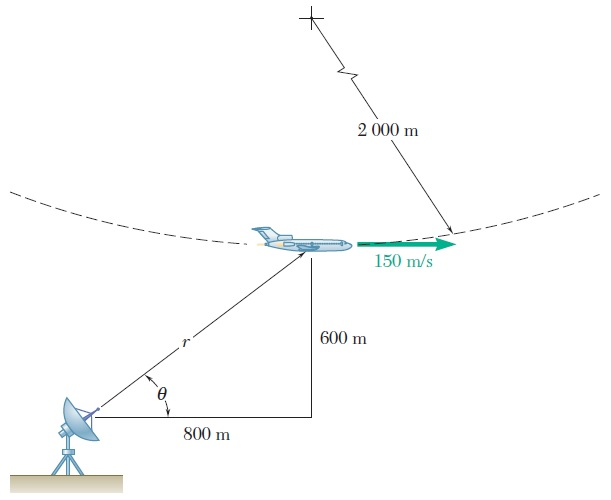
\includegraphics[ width = 0.65\textwidth]{fig_prob_11-193.jpg}
\end{figure}

\end{problem}
\vspace{\baselineskip}

% =============================================
\begin{problem}
Un bloque $A$ de lat\'on (no magn\'etico) de 300 g y un im\'an $B$ de acero de 200 g \linebreak est\'an en equilibrio en un tubo de lat\'on bajo la acci\'on de la fuerza repelente magn\'etica de otro im\'an de acero $C$ ubicado a una distancia $x = 4$ mm de $B$. La fuerza es inversamente proporcional al cuadrado de la distancia entre $B$ y $C$. Si el bloque $A$ se quita repentinamente, determine: 
\begin{enumerate}[label=\alph*.]
\item \textbf{[6 Puntos]} La velocidad m\'axima del bloque $B$. 
\item \textbf{[4 Puntos]} La aceleraci\'on m\'axima del bloque $B$. 
\end{enumerate}
Suponga que la resistencia del aire y la fricci\'on son despreciables. 

\begin{figure}[htb]
\centering
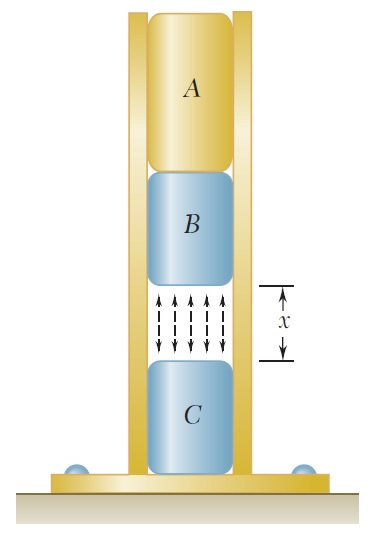
\includegraphics[ width = 0.35\textwidth]{fig_prob_13-37.jpg}
\end{figure}

\end{problem}
\vspace{\baselineskip}

% =============================================
\begin{problem}
\textbf{[6 Puntos]}
Un transportador de sillas est\'a dise\~nado para trasladar 900 esquiadores por hora desde la base $A$ hasta la cumbre $B$. El peso promedio de un esquiador es de 160 lb y la rapidez promedio del transportador es de 250 ft/min. Determine la potencia promedio que requiere el transportador para funcionar. 

\begin{figure}[htb]
\centering
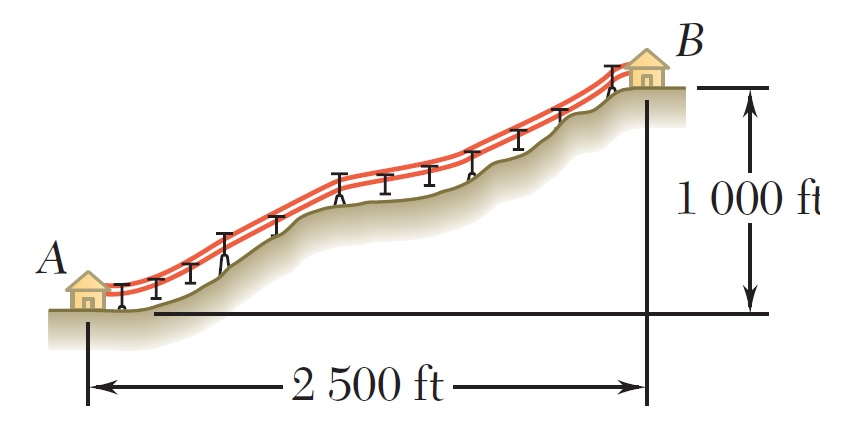
\includegraphics[ width = 0.45\textwidth]{fig_prob_13-48.jpg}
\end{figure}

\end{problem}
\vspace{\baselineskip}

\end{document}
